\documentclass{beamer}

\usetheme{Berlin}

\usecolortheme{dolphin}

\usepackage{amsmath}
\usepackage{graphicx}
\usepackage{setspace}

\title{Spectral Differentiation: Integration and Inversion}
\author{Conor McCoid}
\institute{Simon Fraser University}
\date{February 8th, 2018}

\begin{document}

\frame{\titlepage}

\section{Introduction}

\begin{frame}
\frametitle{Introduction}
\begin{itemize}
\item High order differentiation matrices have round-off error
\item Can we remove sources of round-off error?
\end{itemize}

\begin{block}{Option 1: Preconditioning by integration}
Multiply by integration matrix
\end{block}

\begin{block}{Option 2: Inversion}
Find inverse of linear operator matrix
\end{block}
% Mention that original purpose was to reduce condition number
\end{frame}

\subsection{The collocation method}

\begin{frame}
\frametitle{Chebyshev differentiation matrices [sec.1]}

\begin{columns}

\begin{column}{0.5\textwidth}
\begin{figure}
\includegraphics[width=\textwidth]{ChebDiffMat.pdf}
\end{figure}
\end{column}
% Point out where the round-off error occurs
\begin{column}{0.5\textwidth}
Fig: From pg. 53 of \textit{Spectral Methods in MATLAB} by L.N. Trefethen
\begin{equation*} \label{diff matrix}
\begin{gathered}
D^{(2)} = D \cdot D \\ D^{(k)} = D \cdot D^{(k-1)} = D^k \\
x_k = \cos \left ( \frac{k \pi}{N} \right ) \in [-1,1]
\end{gathered}
\end{equation*}
\end{column}

\end{columns}
\end{frame}

\begin{frame}
\frametitle{The general $m$-th order problem [sec.1]}
\begin{alignat*}{3}
\mathcal{L} u(x) = &  u^{(m)}(x) + \sum_{n = 1}^m q_n(x) u^{(m-n)}(x) = f(x) \\
\mathcal{B}_k u(1) = & \sum_{n = 1}^m a_n^k u^{(m-n)}(1) = a_0^k, && k = && 1,...,k_0 \\
\mathcal{B}_k u(-1) = & \sum_{n = 1}^m a_n^k u^{(m-n)}(-1) = a_0^k, && k = && k_0+1,...,m 
\end{alignat*}
\end{frame}

\begin{frame}
\frametitle{The collocation matrices [sec.1]}
\begin{align*}
\bar{A} = & D^{(m)} + \sum_{n=1}^m Q_n D^{(m-n)}, && Q_n = \begin{bmatrix} q_n(x_0) & & \\ & \ddots & \\ & & q_n(x_N) \end{bmatrix} \\
\hat{A}_k = & \sum_{n=1}^m a_n^k D^{(m-n)}_0, && k = 1,...,k_0 \\
\hat{A}_k = & \sum_{n=1}^m a_n^k D^{(m-n)}_N, && k = k_0+1,...,m
\end{align*}
$D_0^{(m-n)}$ is the first row of $D^{(m-n)}$, $D_N^{(m-n)}$ the last row and $D^{(0)}$ the identity matrix
\end{frame}

\subsection{Combining operator and boundary conditions}

\begin{frame}
\frametitle{Combining $\bar{A}$ and $\hat{A}$ [sec.1]}
$\bar{A}$ and $\hat{A}$ can be concatenated to form the full system:
\begin{equation*}
\begin{bmatrix} \bar{A} \\ \hat{A} \end{bmatrix} \vec{U} = \begin{bmatrix} \vec{f} \\ a_0^1 \\ \vdots \\ a_0^m \end{bmatrix}
\end{equation*}
However, this system may be overdetermined.

Instead, remove rows of $\bar{A}$ and replace them with the rows of $\hat{A}$.
% Why row removal? why not concatenate?
% Can enforce conditions on boundary by ignoring conditions on interior
\end{frame}

\begin{frame}
\frametitle{Combining $\bar{A}$ and $\hat{A}$ [sec.1]}
Each row (and column) of $\bar{A}$ is associated with a Chebyshev node. 

Choose $m$ of these nodes, $V = \{ v_1,...,v_m \}$.

Then the rows associated with these points will be replaced by boundary conditions.

Define a new matrix $A$ by its rows:

\begin{align*}
A_j = \begin{cases} \bar{A}_j & x_j \notin V \\ \hat{A}_k & x_j = v_k \in V \end{cases}
\end{align*}
\end{frame}

\begin{frame}
\frametitle{Combining $\bar{A}$ and $\hat{A}$ [sec.1]}
Alternatively, define the matrices $\tilde{D}^{(k)}$:
\begin{flalign*}
\tilde{D}_j^{(m)} = & \begin{cases} D^{(m)}_j & x_j \notin V \\ \hat{A}_k & x_j = v_k \in V \end{cases} \\
\tilde{D}_j^{(k)} = & \begin{cases} D^{(k)}_j & x_j \notin V \\ 0 & x_j \in V \end{cases}
\end{flalign*}

Then the matrix $A$ is constructed just like $\bar{A}$:
\begin{equation*}
A = \tilde{D}^{(m)} + \sum_{n=1}^m Q_n \tilde{D}^{(m-n)}
\end{equation*}
\end{frame}

\section{Integration}

\subsection{Preconditioning}

\begin{frame}
\frametitle{Preconditioning [sec.2]}
$\tilde{D}^{(m)}$ is a large source of round-off error.

We would like to remove it by multiplying $A$ by some matrix $B$:
\begin{equation*}
B A = I + \sum_{n=1}^m B Q_n \tilde{D}^{(m-n)}
\end{equation*}
Usually, $B \tilde{D}^{(m)} \approx I$ is enough.

In our case, we hope to find $\tilde{D}^{(m)} B = I$.
\end{frame}

\begin{frame}
\frametitle{Integration matrix [sec.2]}
If the columns of $B$ are representations of polynomials $B_j(x)$, then:
\begin{align*}
\tilde{D}^{(m)}_i \vec{B}_j = & \begin{cases} B^{(m)}_j(x_i) & x_i \notin V \\ \mathcal{B}_k B_j(\pm 1) & x_i = v_k \in V \end{cases} \\
 \implies B^{(m)}_j(x_i) = & \begin{cases} \delta_{ij} & x_j \notin V \\ 0 & x_j \in V \end{cases} \\
\mathcal{B}_k B_j(\pm 1) = & \begin{cases} 1 & x_j = v_k \in V \\ 0 & x_j \neq v_k \end{cases}
\end{align*}
% Mention that V is the new contribution?
\end{frame}

\subsection{The Chebyshev polynomials}

\begin{frame}
\frametitle{The Chebyshev polynomials [sec.1]}

\begin{columns}

\begin{column}{0.4\textwidth}
\begin{figure}
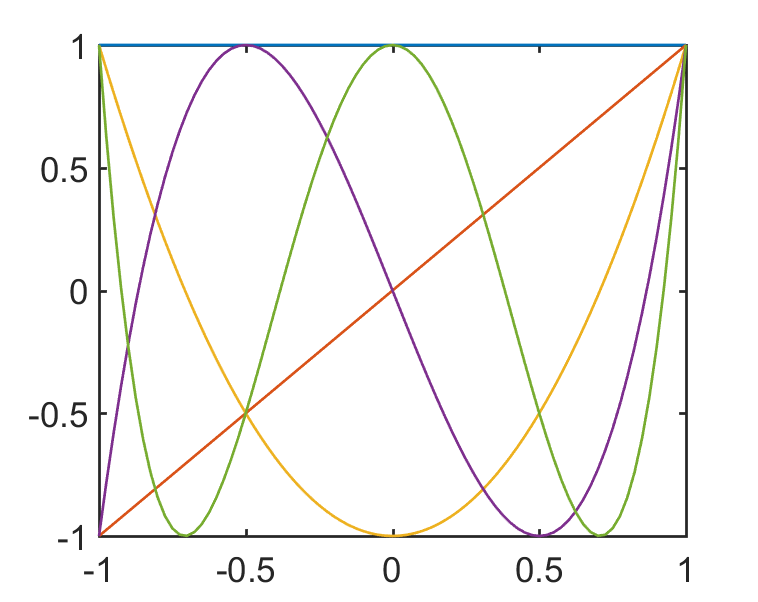
\includegraphics[width=\textwidth]{ChebPoly.png}
\caption{$T_k(x) = \cos \left ( k \arccos (x) \right )$}
\end{figure}
\end{column}

\begin{column}{0.6\textwidth}
\begin{align*}
 \partial_x^{-1} T_0(x) = & T_1(x) \\
 \partial_x^{-1} T_1(x) = & T_2(x) / 4 \\
 \partial_x^{-1}T_k(x) = & \frac{1}{2} \left ( \frac{T_{k+1}(x)}{k+1} - \frac{T_{k-1}(x)}{k-1} \right ).
\end{align*}
\end{column}

\end{columns}
\end{frame}

\begin{frame}
\frametitle{The Chebyshev polynomials [sec.1]}
$T_k(x)$ satisfy a discrete orthogonality relation on the nodes:
\begin{equation*}
\begin{gathered}
\langle T_k,T_j \rangle_c = 
\sum_{i=0}^{N} \frac{1}{c_i} T_k(x_i) T_j(x_i) = \frac{c_j}{2} N \delta_{jk} \\
c_j = \begin{cases} 2 \quad k = 0, N \\ 1 \quad 1 \leq k < N \end{cases}
\end{gathered}
\end{equation*}
\end{frame}

\subsection{Constructing the preconditioner}

\begin{frame}
\frametitle{Decomposing $B_j(x)$ [sec.2] (adapted from Wang et al.)}
$B_j(x)$ is a polynomial of at most degree $N$, then its $m$-th derivative can be represented as
\begin{equation*}
\begin{gathered}
 B^{(m)}_j(x) = \sum_{k=0}^N b_{k,j} T_k(x), \quad b_{k,j} = 0 \quad \forall \quad k=N-m+1,...,N \\
\langle B^{(m)}_j,T_k \rangle_c = b_{k,j} c_k N / 2
\end{gathered}
\end{equation*}
Let $\beta_{k,j} = B^{(m)}_j(v_k)/c_n$ where $v_k = x_n \in V$; these values are unknown
\begin{equation*}
b_{k,j} = \frac{2}{c_k N} \langle B_j^{(m)}, T_k \rangle_c = \frac{2}{c_k N} \left ( \frac{1}{c_j} T_k(x_j) + \sum_{n=1}^m \beta_{n,j} T_k(v_n) \right ).
\end{equation*}
\end{frame}

\begin{frame}
\frametitle{Solving for $\beta_{k,j}$ [sec.2]}
Since $b_{k,j} = 0$ for $k = N-m+1,...,N$, we can make a system to solve for $\beta_{k,j}$:
\begin{equation*}
\begin{bmatrix} T_N(v_1) & \dots & T_N(v_m) \\ \vdots & \ddots & \vdots \\ T_{N-m+1}(v_1) & \dots & T_{N-m+1}(v_m) \end{bmatrix}
\begin{bmatrix} \beta_{1,j} \\ \vdots \\ \beta_{m,j} \end{bmatrix} = 
- \frac{1}{c_j} \begin{bmatrix} T_N(x_j) \\ \vdots \\ T_{N-m+1}(x_j) \end{bmatrix}
\end{equation*}
\end{frame}

\begin{frame}
\frametitle{Boundary conditions [sec.2]}
For $x_j \notin V$
\begin{align*}
B_j(x) = & \sum_{k=0}^{N-m} b_{k,j} \left ( \partial_x^{-m} T_k(x) - p_{k}(x) \right ) \\
\mathcal{B}_n p_{k}(\pm 1) = & \mathcal{B}_n \partial_x^{-m} T_k(\pm 1)
\end{align*}
For $x_j \in V$, $B_j(x)$ is a polynomial of degree at most $m-1$ satisfying
\begin{equation*}
\mathcal{B}_k B_j(\pm1) = \begin{cases} 1 & x_j = v_k \\ 0 & x_j \neq v_k \end{cases}
\end{equation*}
\end{frame}

\section{Inversion}

\begin{frame}
\frametitle{Inversion matrices [sec.3]}
\begin{equation*}
A = \tilde{D}^{(m)} + \sum_{n=1}^m Q_n \tilde{D}^{(m-n)}
\end{equation*}
We want $R$ such that $AR = I$.
If $R_j(x)$ is the polynomial represented by the $j$-th column of $R$, then:
\begin{align*}
\mathcal{L} R_j(x_i) = & \begin{cases} \delta_{ij} & x_j \notin V \\ 0 & x_j \in V \end{cases} \\
\mathcal{B}_k R_j(\pm 1) = & \begin{cases} 0 & x_j \neq v_k \in V \\ 1 & x_j = v_k \in V \end{cases}
\end{align*}
\end{frame}



\section{Examples}

\begin{frame}
\frametitle{Methods}
Standard:
\begin{equation*}
A U = F
\end{equation*}
Preconditioning (generalized from Wang et al.):
\begin{equation*}
\left ( I + \sum_{n=1}^m B Q_n \tilde{D}^{(m-n)} \right ) U = B F
\end{equation*}
Inverse operator (new):
\begin{equation*}
U = R F
\end{equation*}
\end{frame}

\subsection{Singular example}

\begin{frame}
\frametitle{Singular example: function of $V$ [sec.6.1] }
\begin{figure}
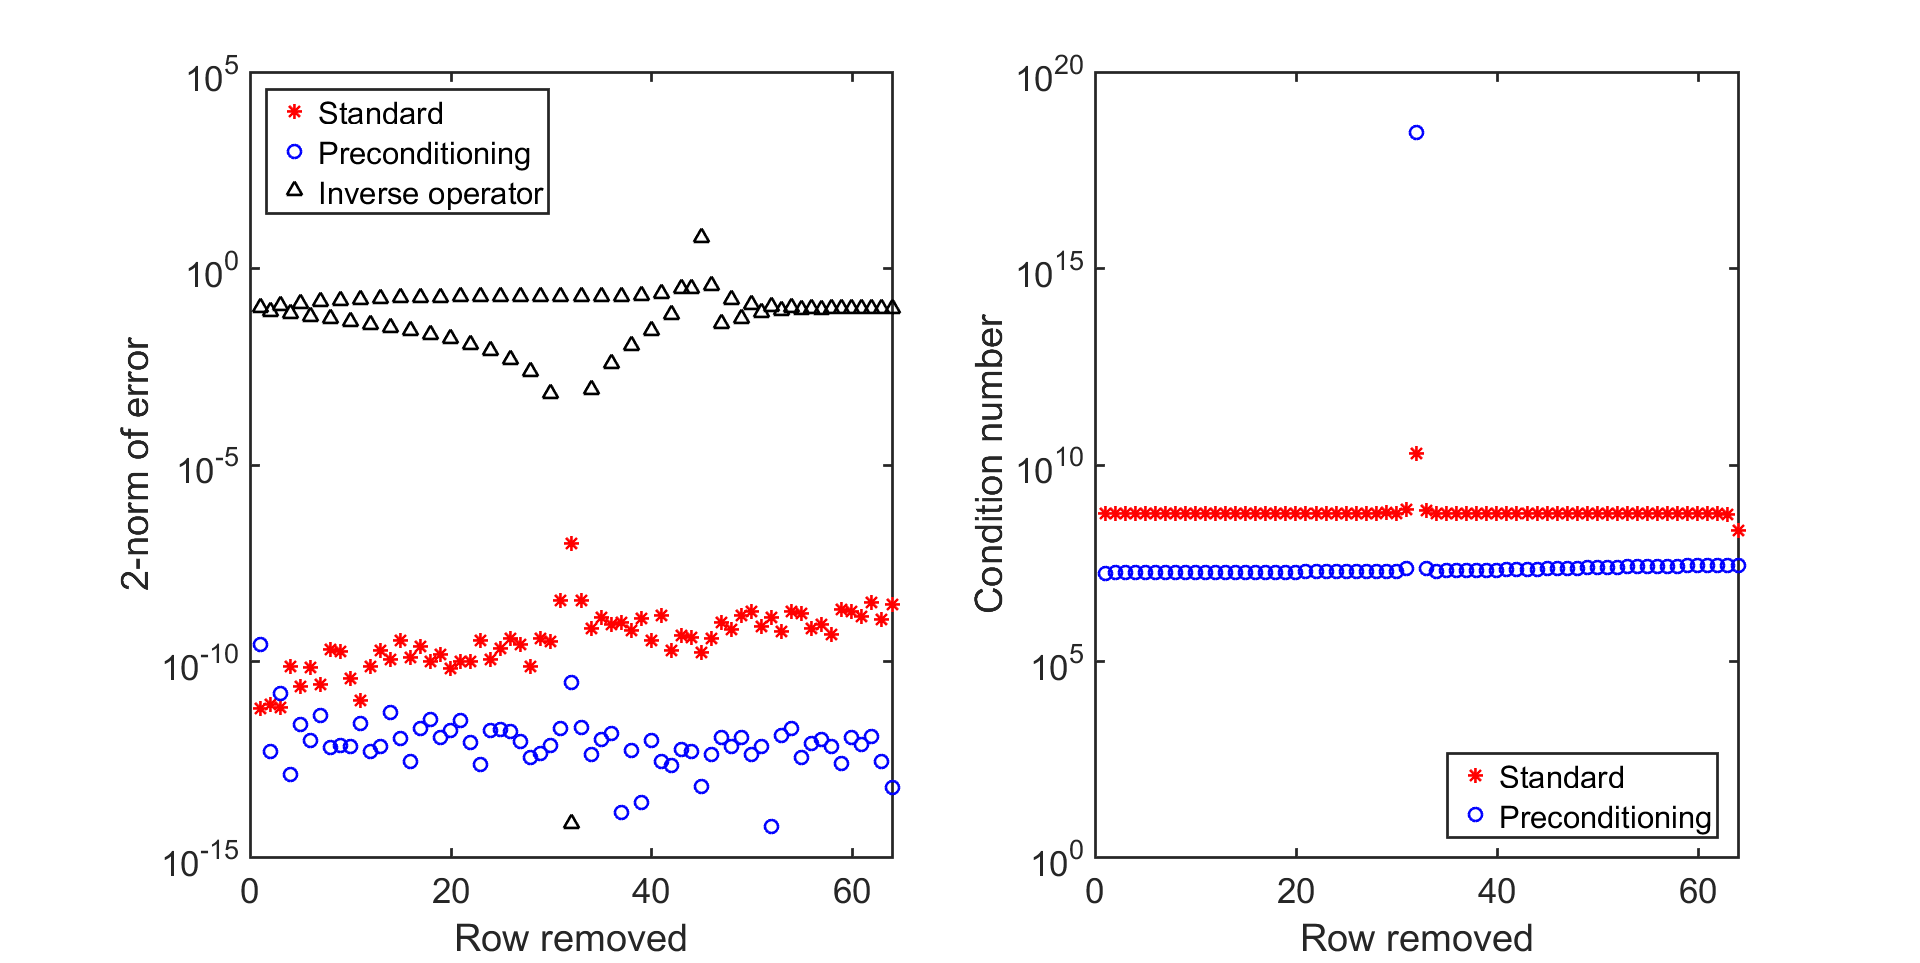
\includegraphics[width=0.9\textwidth]{example_SingCoeffs_02.png}
\caption{$x u''(x) - (x+1) u'(x) + u(x) = x^2, \quad u(\pm 1) = 1$}
\end{figure}
\end{frame}

\begin{frame}
\frametitle{Singular example: function of $N$ [sec.6.1] }
\begin{figure}
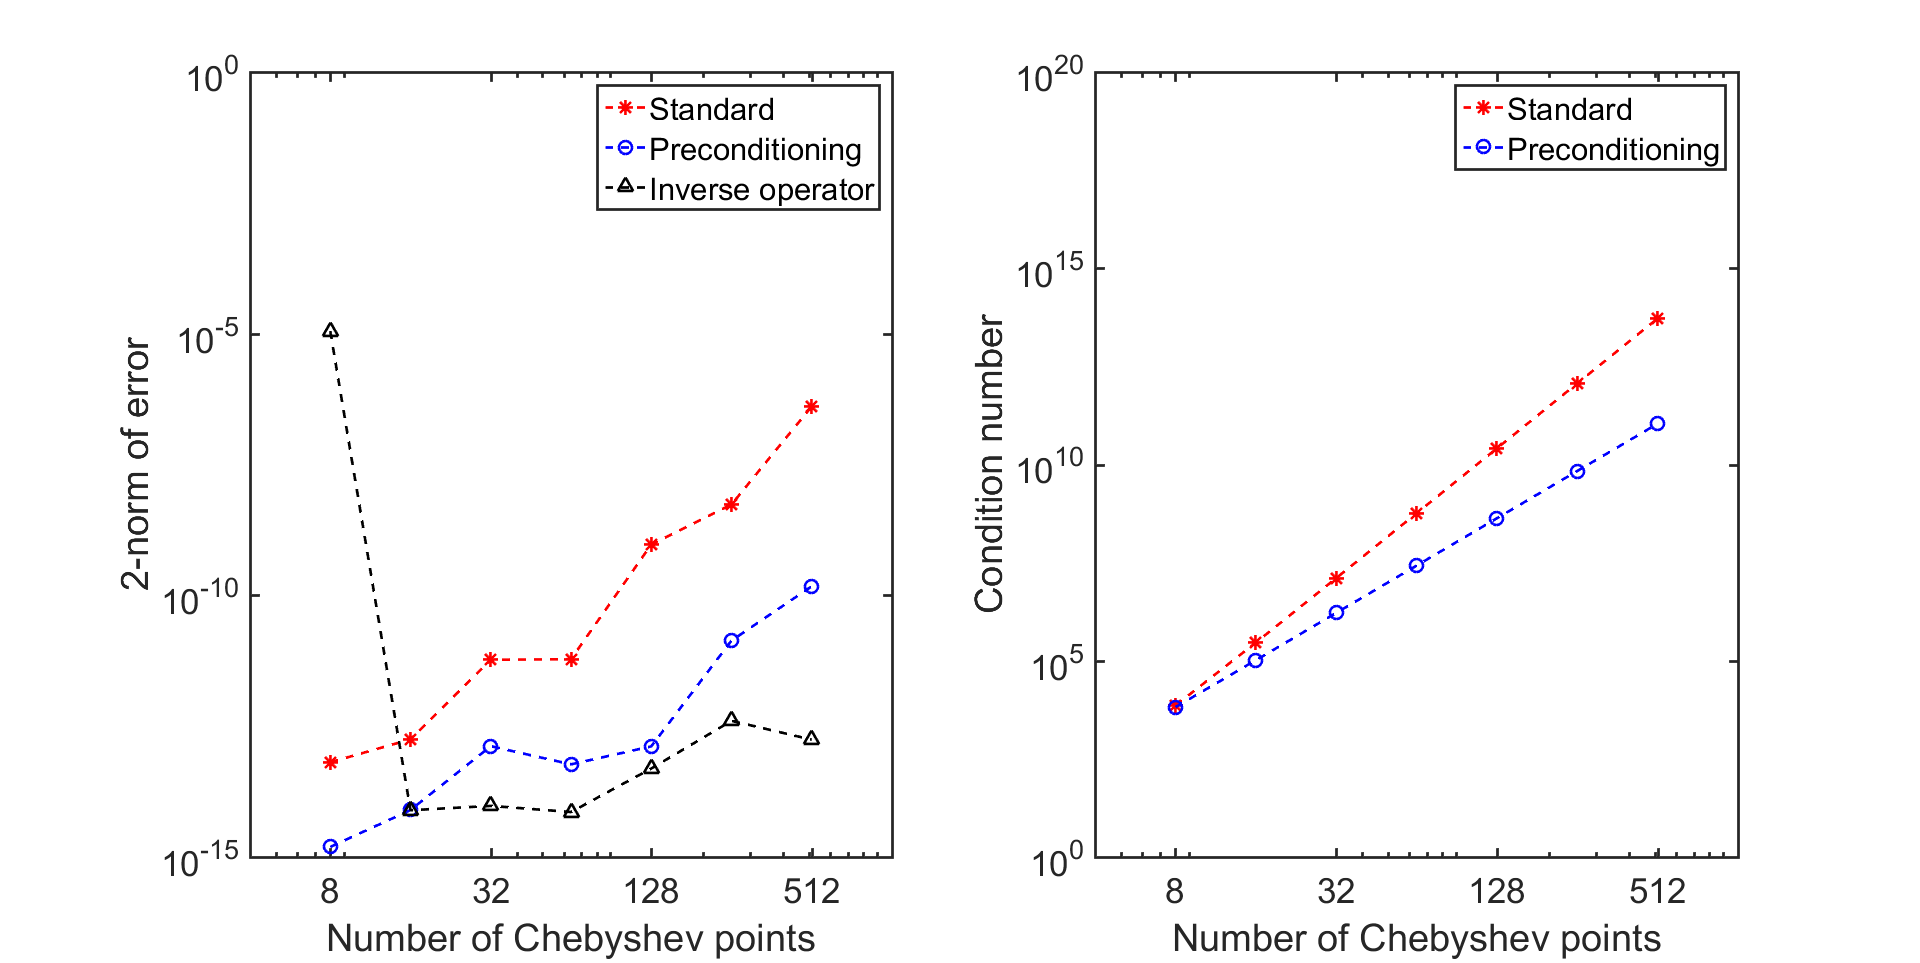
\includegraphics[width=0.9\textwidth]{example_SingCoeffs_03.png}
\caption{$x u''(x) - (x+1) u'(x) + u(x) = x^2, \quad u(\pm 1) = 1$}
\end{figure}
\end{frame}

\subsection{Constant coefficients}

\begin{frame}
\frametitle{Constant coefficients: function of $V$ [sec.6.2] }
\begin{figure}
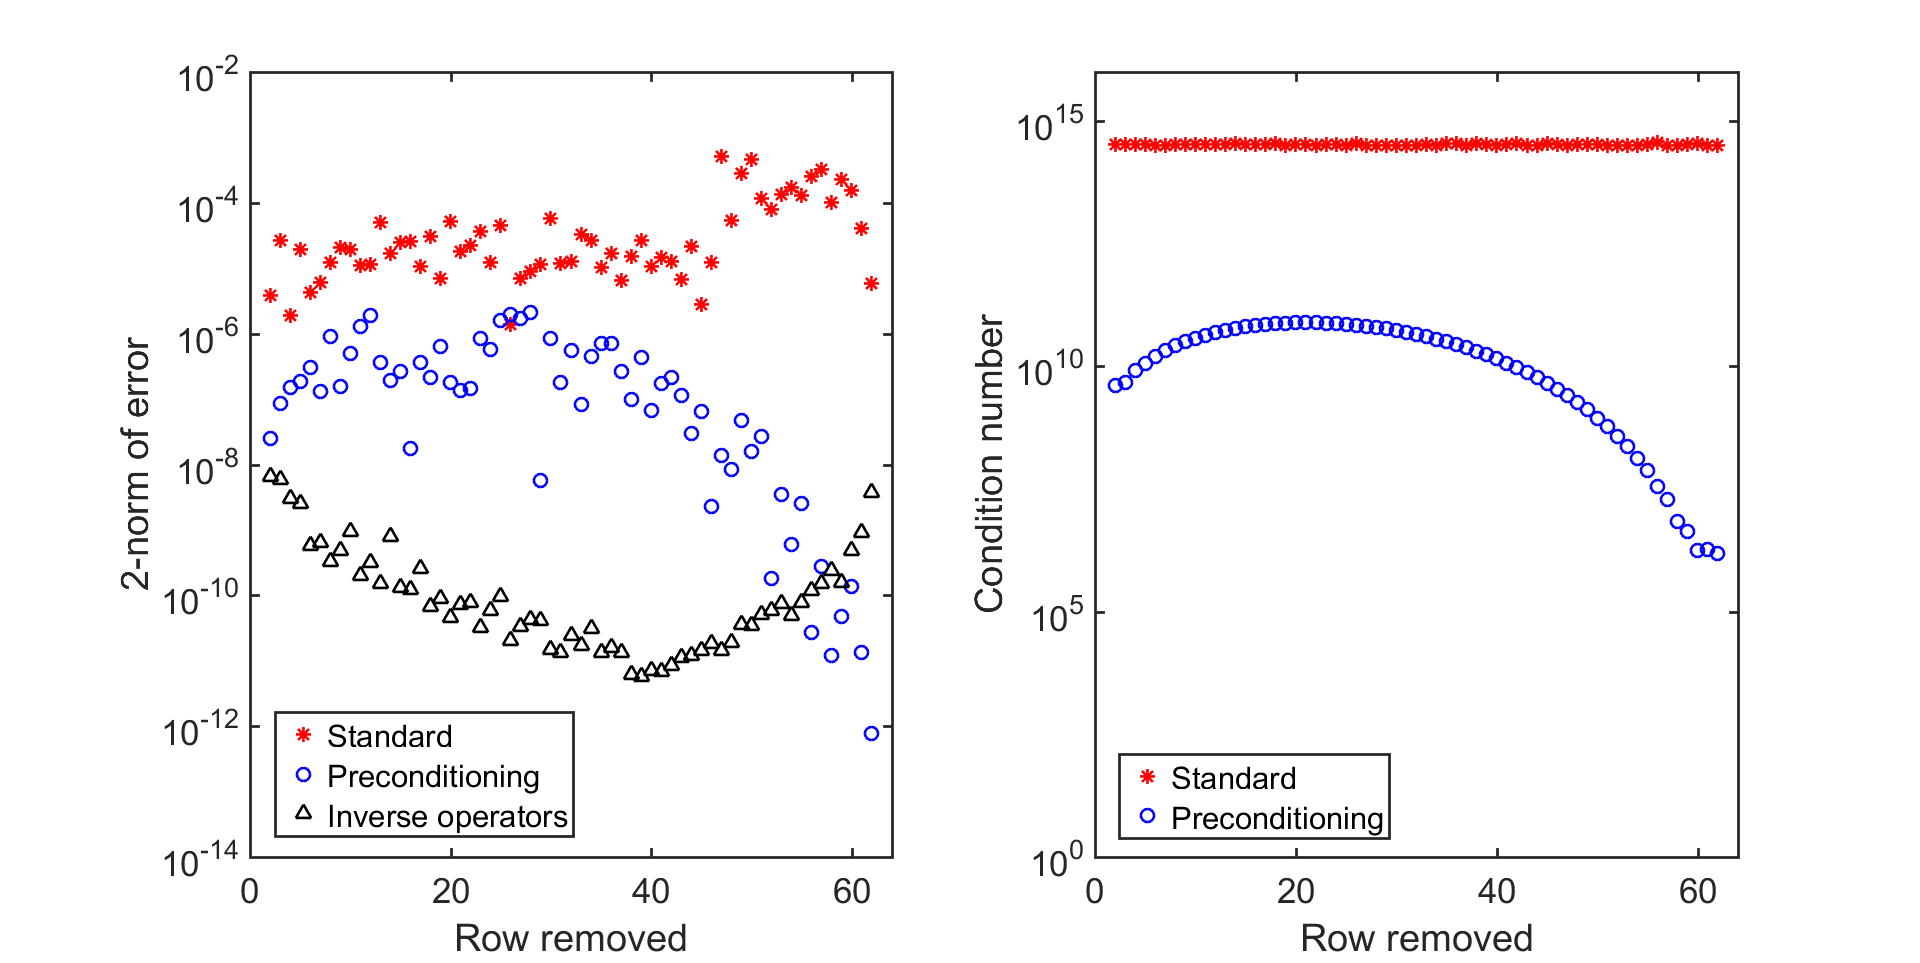
\includegraphics[width=0.9\textwidth]{example_5thCC_V.png}
\caption{$u^{(5)}(x) + u^{(4)}(x) - u'(x) - u(x) = f(x)$}
\end{figure}
\end{frame}

\begin{frame}
\frametitle{Constant coefficients: function of $N$ [sec.6.2]}
\begin{figure}
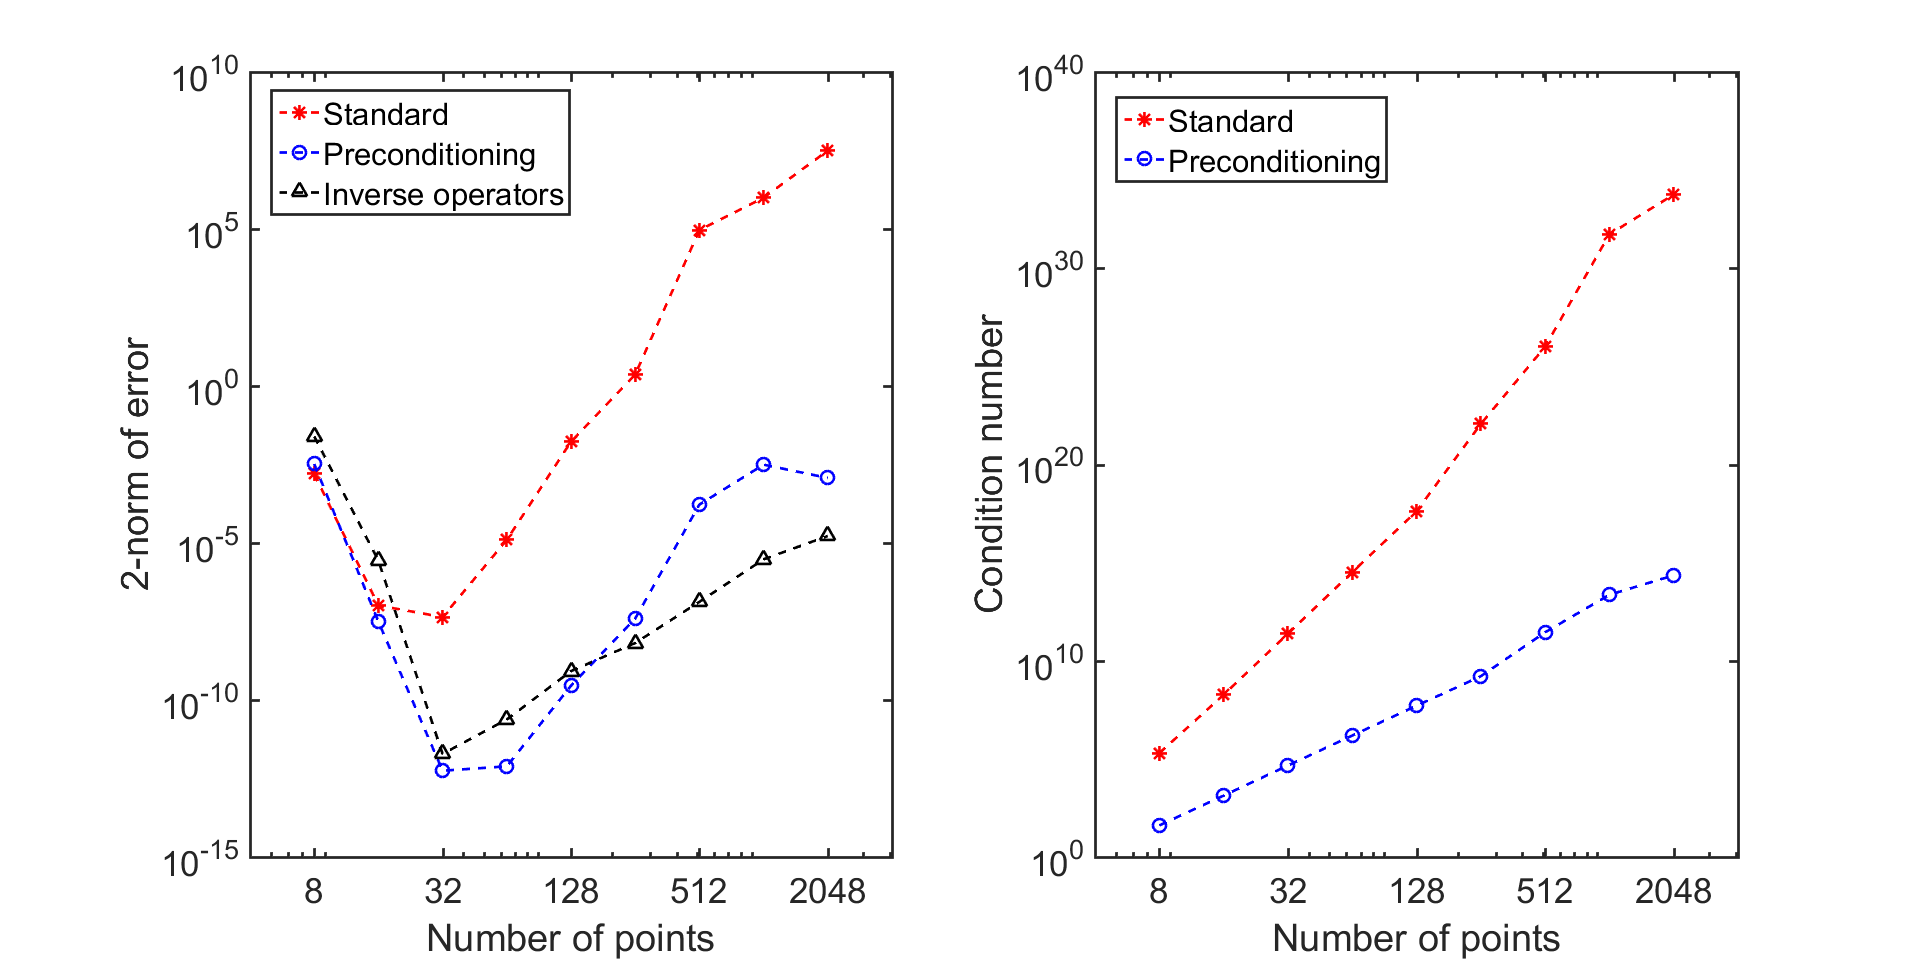
\includegraphics[width=0.9\textwidth]{example_5thCC_N.png}
\caption{ $u^{(5)}(x) + u^{(4)}(x) - u'(x) - u(x) = f(x)$}
\end{figure}
\end{frame}

\subsection{Nonconstant coefficients}

\begin{frame}
\frametitle{Nonconstant coefficients: function of $V$ [sec.6.3]}
\begin{figure}
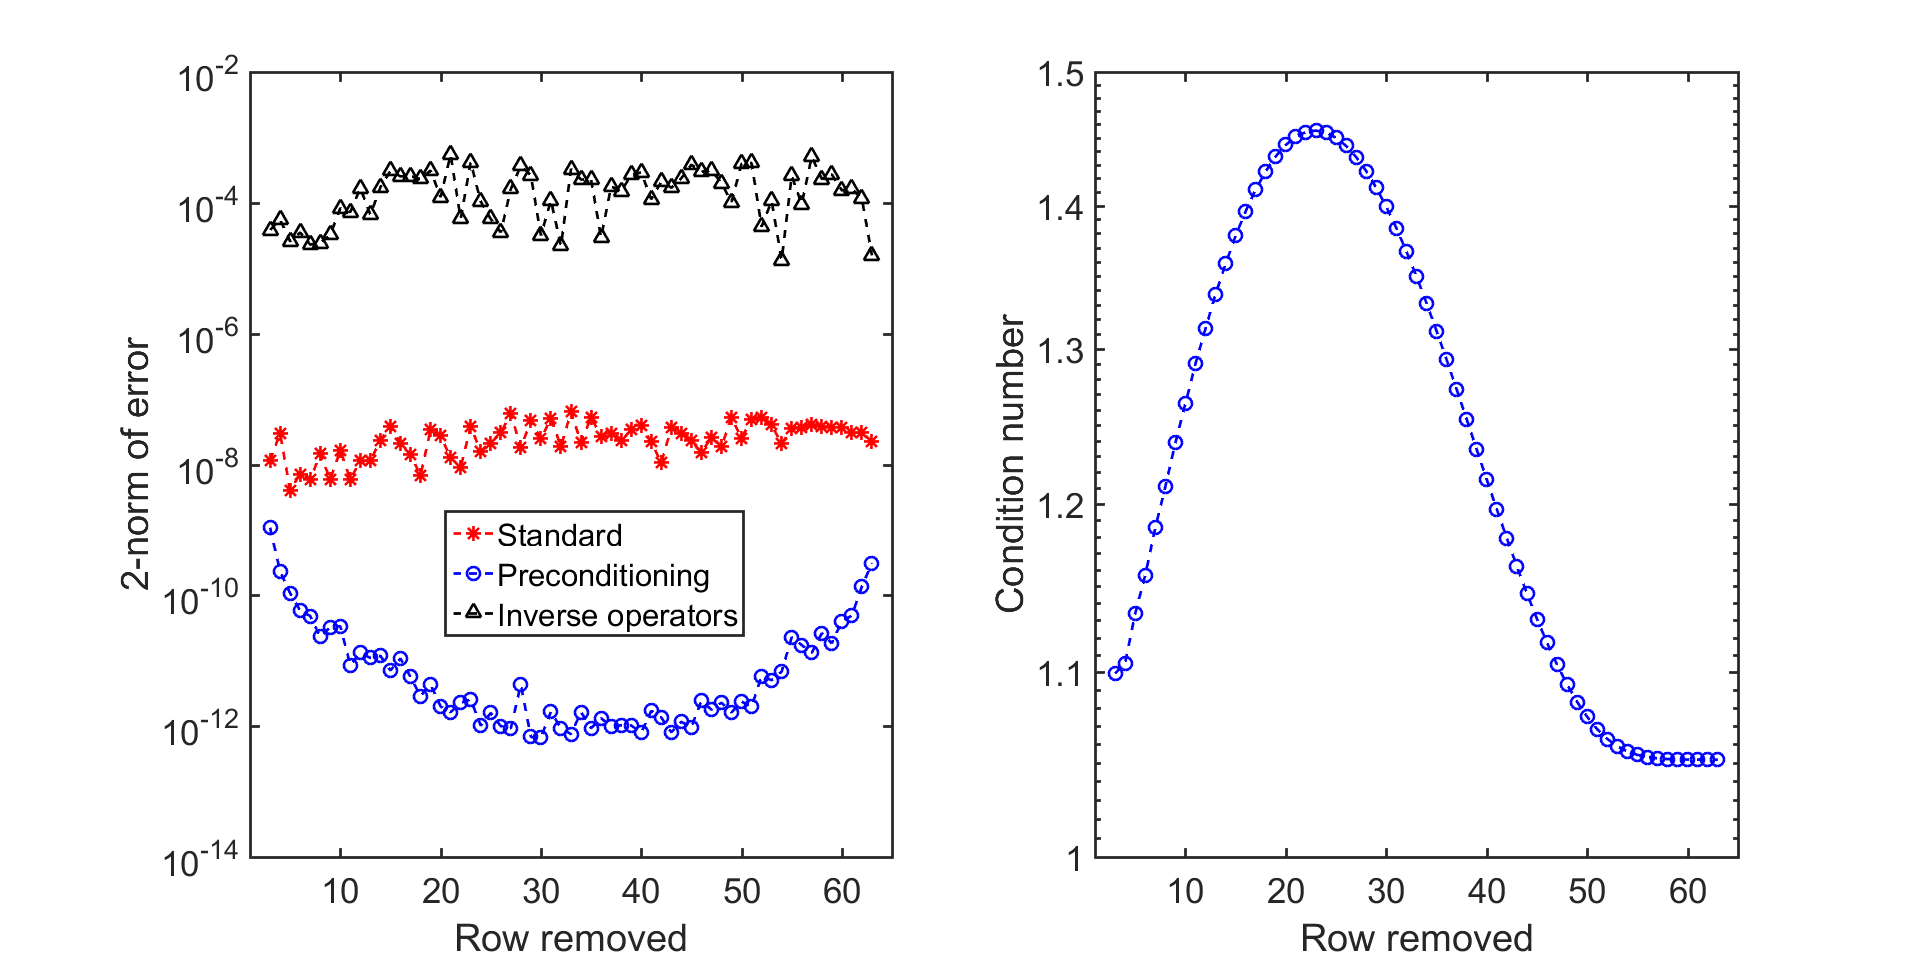
\includegraphics[width=0.9\textwidth]{example_Wang5th_V64.png}
\caption{ $u^{(5)}(x) + \sin(10x) u'(x) + x u(x) = f(x), \quad u(\pm 1) = u'(\pm 1) = u''(1) = 0$}
\end{figure}
\end{frame}

\begin{frame}
\frametitle{Nonconstant coefficients: function of $N$ [sec.6.3]}
\begin{figure}
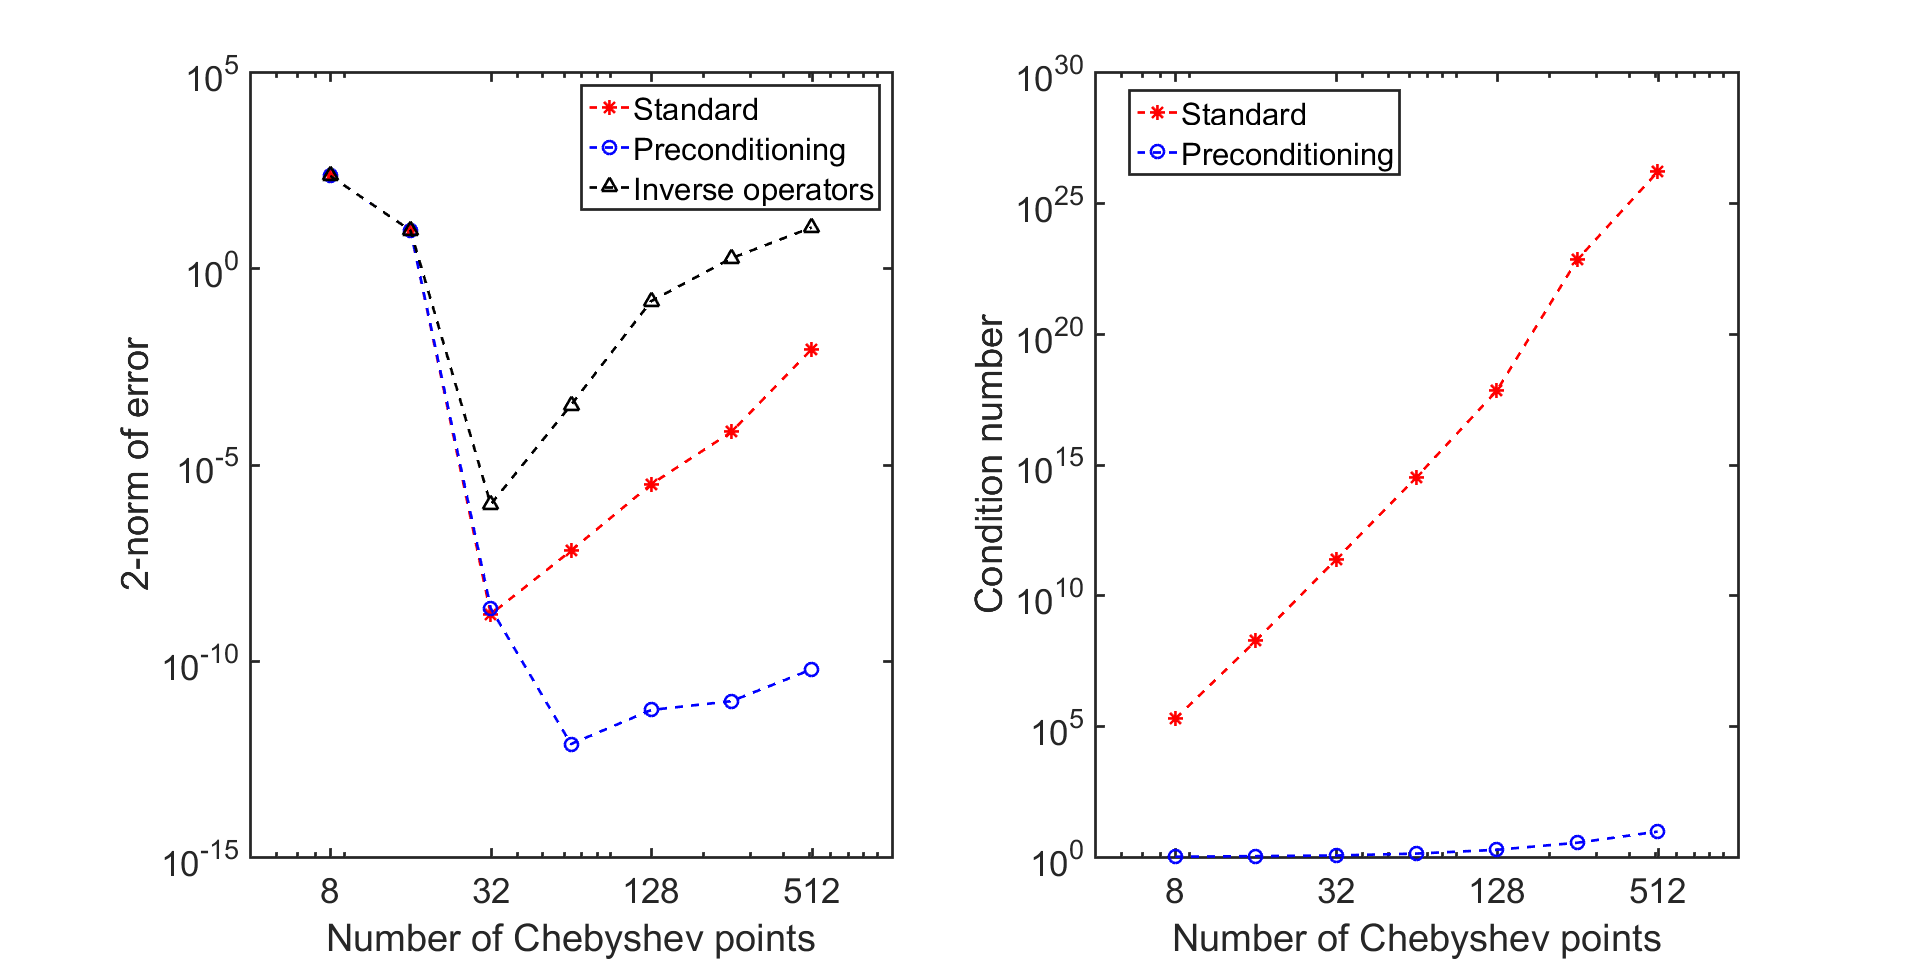
\includegraphics[width=0.9\textwidth]{example_Wang5th_N.png}
\caption{$u^{(5)}(x) + \sin(10x) u'(x) + x u(x) = f(x), \quad u(\pm 1) = u'(\pm 1) = u''(1) = 0$}
\end{figure}
\end{frame}

\subsection{Nonlinear example}

\begin{frame}
\frametitle{Nonlinear [sec.6.4]}
\begin{figure}
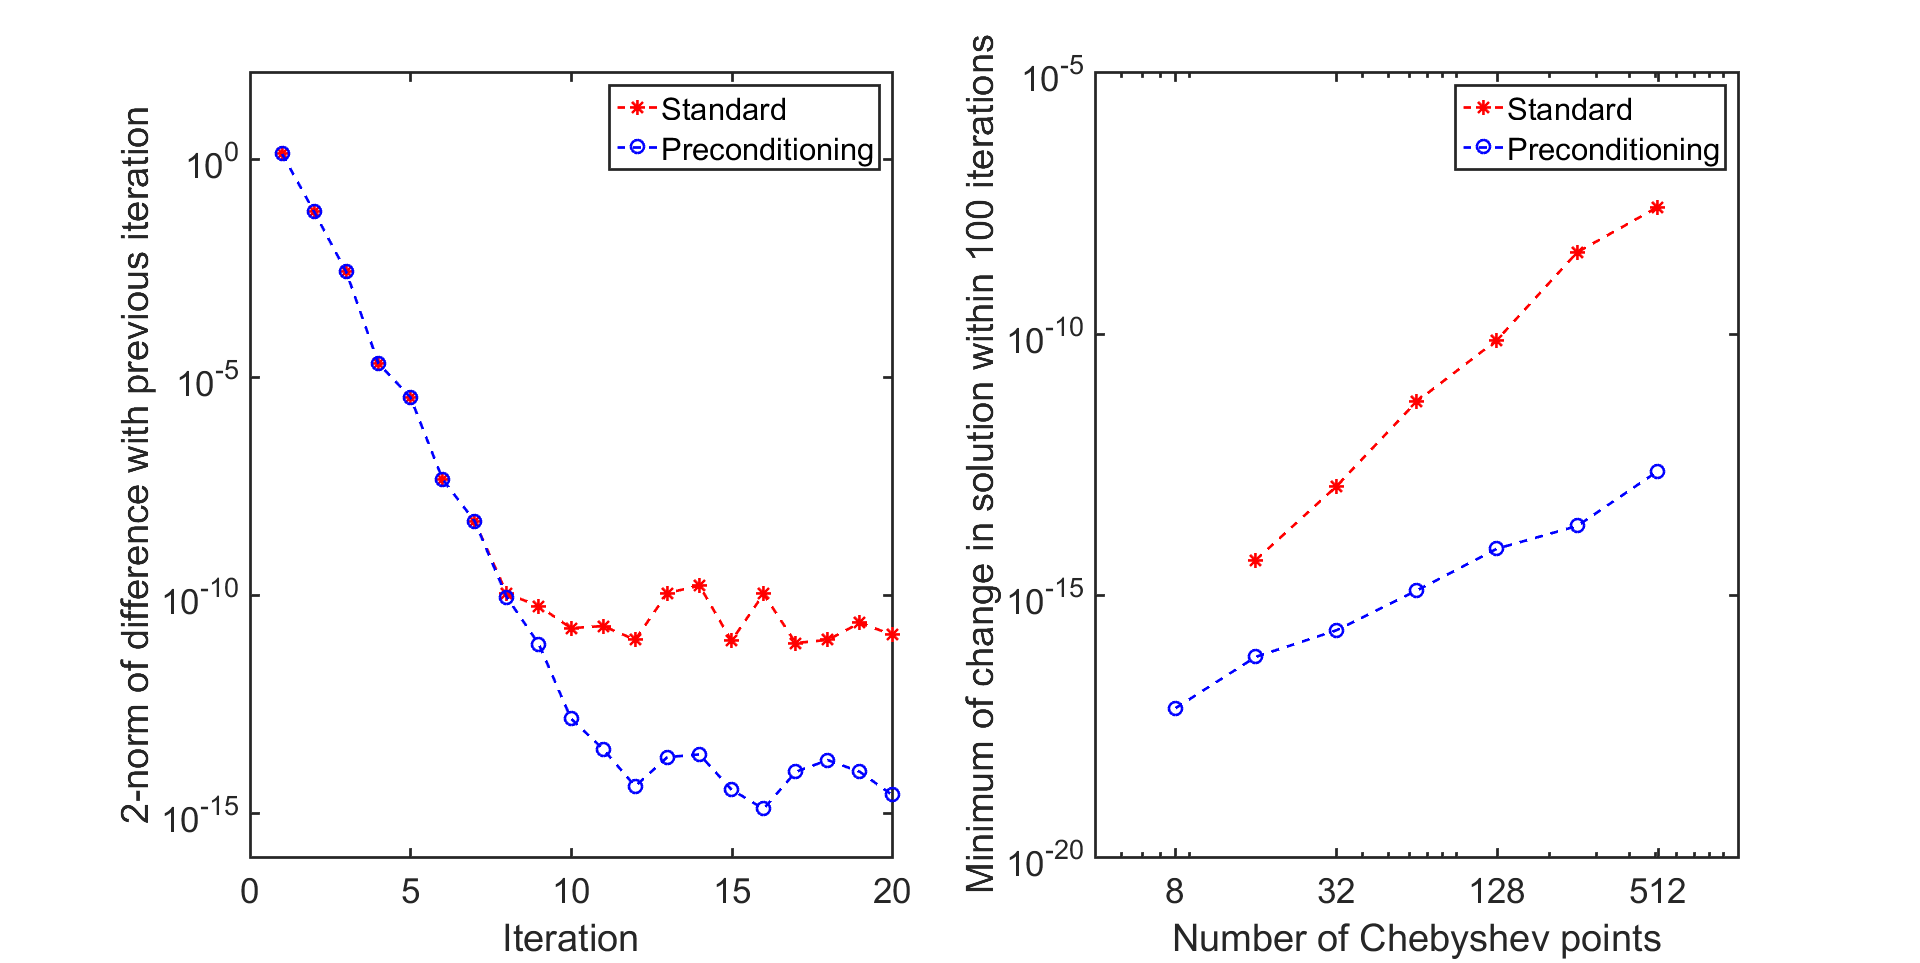
\includegraphics[width=0.9\textwidth]{example_AscherNonlinear.png}
\caption{ $u^{(4)}(x) = u'(x) u''(x) - u(x) u^{(3)}(x)$, $ u(\pm 1) = u'(-1) = 0, \quad u'(1) = 1 $}
\end{figure}
\end{frame}

\section{Conclusion}

\begin{frame}
\frametitle{Conclusion}
\begin{itemize}
\item Some sources of round-off error (largest order derivative) are easy to remove
\item Remaining derivatives prove challenging
\item Inversion operators need homogeneous solutions, which may not be available
\end{itemize}
\end{frame}

\begin{frame}
\frametitle{Future Works}
\begin{itemize}
\item A priori row removal
\item Alternative methods to calculate integration matrix
\item Inversion for constant coefficients
\item Preconditioning for perturbed/ boundary layer problems
\end{itemize}
\end{frame}

\begin{frame}
% Move this slide to the end
\frametitle{Variation of parameters [sec.3]}
\begin{equation*}
\begin{gathered}
R_j(x) = \sum_{k=1}^m G_{k,j}(x) P_k(x) \\
\sum_{k=1}^m G_{k,j}'(x) P_k^{(l)}(x) = 0 \quad l = 0,...,m-2 \\
G_{k,j}'(x_i) = \begin{cases} \beta_{k,j} & x_i = x_j \\ 0 & x_i \neq x_j, v_k \end{cases} \\
\mathcal{L} P_k(x) = 0, \quad P_k^{(l)}(v_k) = \begin{cases} 0 & l < m \\ 1 & l =m \end{cases}
\end{gathered}
\end{equation*}
\end{frame}

\end{document}